\documentclass[portrait,a0paper]{baposter}

\usepackage{calc}
\usepackage{url}
\usepackage{amsmath}
\usepackage{amssymb}
\usepackage{relsize}
\usepackage{multirow}
\usepackage{booktabs}
\usepackage{graphicx}
\usepackage{multicol}
\usepackage[T1]{fontenc}
\usepackage{ae}
\usepackage{mathrsfs}
\usepackage{ifpdf}
\usepackage{wallpaper}

\renewcommand{\familydefault}{\sfdefault}

\ifpdf
	\pdfcompresslevel=9
	\pdfinfo
	{
		/Author (Luis Sanabria-Russo, Jaume Barcel\'{o}, Boris Bellalta)
		/Title (Fairness in Collision-Free WLANs)
		/Subject (Poster for INFOCOM 2013)
	}
\fi

\selectcolormodel{cmyk}

\definecolor{imdeanavy}{cmyk}{1,0.342,0,0.714}
%\definecolor{imdeabluedark}{cmyk}{0.628,0.345,0,0.431}
\definecolor{imdeabluedark}{cmyk}{0.23,0.11,0,0.33}
\definecolor{imdeabluelight}{cmyk}{0.372,0.208,0,0.114}
\definecolor{imdeacyan}{cmyk}{0.091,0.050,0,0.055}

\newenvironment{packeditemize}{
\begin{itemize}
	\setlength{\itemsep}{1pt}
	\setlength{\parskip}{0pt}
	\setlength{\parsep}{0pt}
}{\end{itemize}}

\begin{document}

\background
{
\begin{tikzpicture}[remember picture,overlay]%
\draw (current page.north west)+(-3.9pt,3.5pt) node[anchor=north west]
{
		\ifpdf
			
\includegraphics[width=\paperwidth+0.7pt]{background2-eps-converted-to.pdf}\\
		\else
			
\includegraphics[width=\paperwidth+0.7pt]{background2.eps}\\
		\fi
};
\end{tikzpicture}%
}

\begin{poster}
% Settings
{
	grid=no,
	columns=2,
	colspacing=1em,
	eyecatcher=no,
	borderColor=imdeanavy,
	textborder=rectangle,
  	titleColor=white,
    	authorColor=white,
	headerfont=\textsf,
	headerborder=closed,
	headershape=rectangle,
	headerColorOne=imdeabluedark,
	headerColorTwo=imdeabluedark,
	headerFontColor=white,
	boxColorOne=white,
	boxColorTwo=imdeacyan,
	boxshade=shade-tb,
	background=user,
	bgColorOne=imdeacyan,
	bgColorTwo=imdeabluelight,
	headerheight=0.12\textheight,
	linewidth=1pt
}
% Eye Catcher
{
}
% Title
{Fairness in Collision-Free WLANs}
% Authors
{
	Luis Sanabria-Russo, Jaume Barcel{\'o}, Boris Bellalta\vspace{0.5em}\\
	\normalsize Universitat Pompeu Fabra, Barcelona, Spain
}
% Logo
% {
% \begin{minipage}{17em}
% 	\begin{center}
% 		\ifpdf
% 			
\includegraphics[width=15em]{NeTS-logo-eps-converted-to.pdf}\\
% 		\else
% 			
\includegraphics[width=15em]{NeTS-logo.eps}\\
% 		\fi
% 	\end{center}
% \end{minipage}
% }

\headerbox{Motivation}{name=motivation,column=0,row=0,span=2}
{

Wireless networks are composed of nodes that must contend for the medium in a distributed manner. If it two or more contenders attempt transmission at the same time, a collision occurs. %Collisions are intelligible for the receiver, forcing colliding nodes to restart the contention for the medium.

Collisions are the main cause of throughput degradation in wireless local area networks (WLANs), so by constructing collision-free WLANs one can attain greater levels of throughput.

% \begin{itemize}
%  \item What is a contention protocol for?: explain that the medium is shared.
%  \item Highlight that it is widely used by current WiFi devices.
%  \item What are the repercussions of a collision?
% \end{itemize}

}

\headerbox{CSMA/CA}{name=contention,column=0,below=motivation}{

Carrier Sense Multiple Access with Collision Avoidance (CSMA/CA) is the most widely used protocol for medium access control (MAC) in WLANs. CSMA/CA's job is to coordinate access to the medium for each contender.
\\\\
Time in WLANs is slotted, so CSMA/CA divides it into empty, collision and successful transmission time slots. When a node has something to transmit, it picks a random backoff counter $B\in[0,CW(k)-1]$, where $k\in[0,\ldots,m]$ is the \emph{backoff stage} and $CW(k)=2^{k}CW_{\min}$ is the contention window, with $CW_{\min}$ its minimum value.
Each passing empty slot decrements $B$ by one. Contenders attempt transmission when the counter expires ($B=0$).

%It might be appropriate to detail the behavior of CSMA/CA and CSMA/ECA. A balls and bins figure?

\begin{center}
\begin{tikzpicture}
\path
	\ifpdf
		(0,0) node{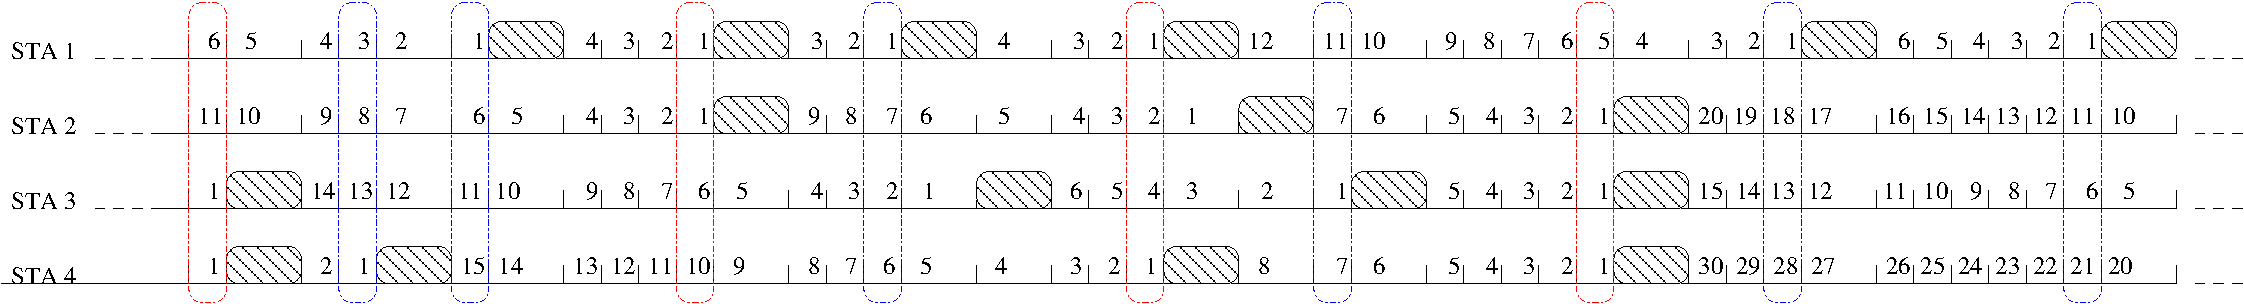
\includegraphics[width=\linewidth]{csma_ca-eps-converted-to.pdf}}
	\else
		(0,0) node{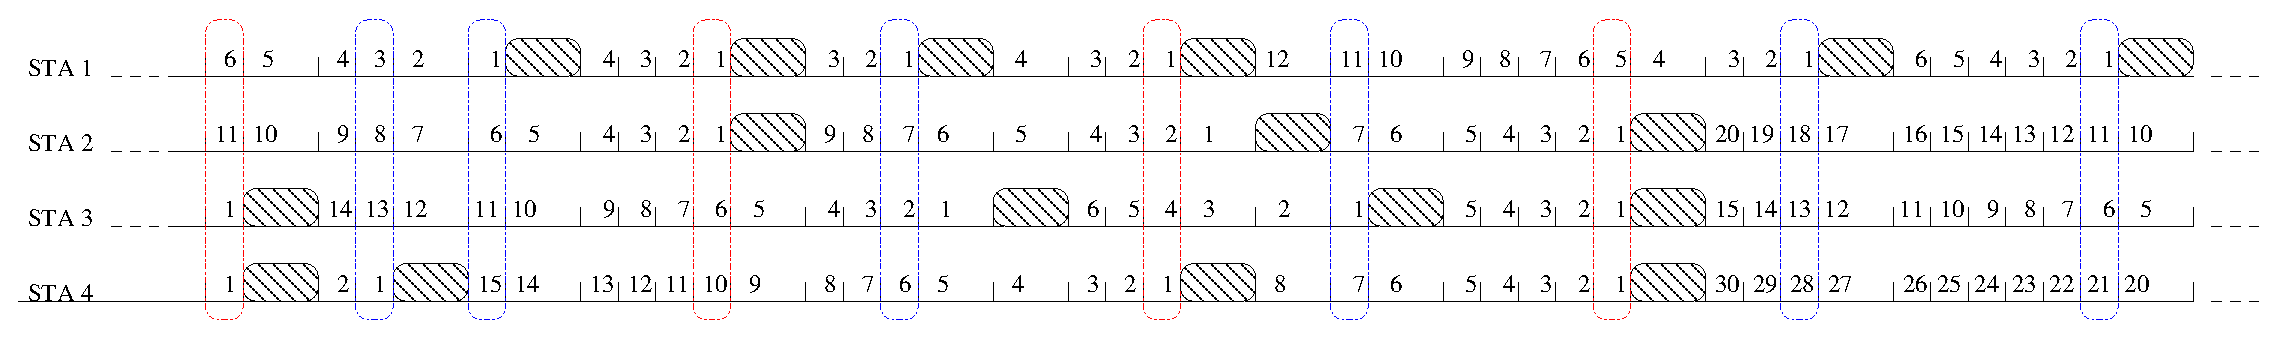
\includegraphics[width=\linewidth]{csma_ca.eps}}
	\fi
	(0,-1.3) node {\smaller Example CSMA/CA behavior.};
\end{tikzpicture}
\end{center}

If a contender collides, it doubles the range of possible values whence it draws $B$ by incrementing the backoff stage ($k$) in one. This measure effectively reduces the collision probability.
After a successful transmission, the contender resets is backoff stage ($k=0$).
}

\headerbox{Basic ECA}{name=hysteresis,column=0,below=contention}{

% This section introduces the hysteresis and fair share concepts, namely:
% \begin{itemize}
% 	\item How is it possible to allocated more contenders in a collision-free fashion?
% 	\item What are the repercussions related to fairness?
% 	\item How fair share solves this issue?
% \end{itemize}

CSMA/CA relies in a random backoff counter ($B$) that by its nature generates collisions. Furthermore, it instructs nodes to reset the backoff stage ($k$) after a successful transmission: increasing the collision probability. Basic Carrier Sense Multiple Access with Enhanced Collision Avoidance~\cite{CSMA_ECA} (Basic ECA) achieves a collision-free state by picking a deterministic backoff counter $B_{d}=CW_{\min}/2$ after successful transmissions. This choice makes it possible for CSMA/ECA to fairly coexist with CSMA/CA.
\\\\
By picking a deterministic backoff counter and achieving a collision-free state, Basic ECA is capable of throughput levels beyond those attained with CSMA/CA.

\begin{center}
\begin{tikzpicture}
\path
	\ifpdf
		(0,0) node{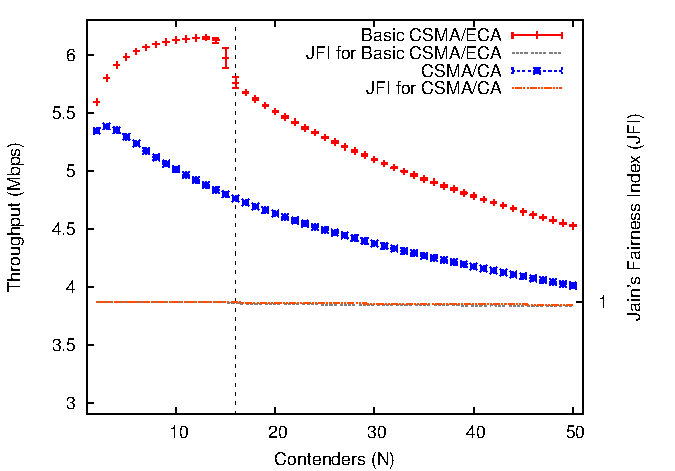
\includegraphics[width=\linewidth]{ECA-vs-CA-FINAL-eps-converted-to.pdf}}
	\else
		(0,0) node{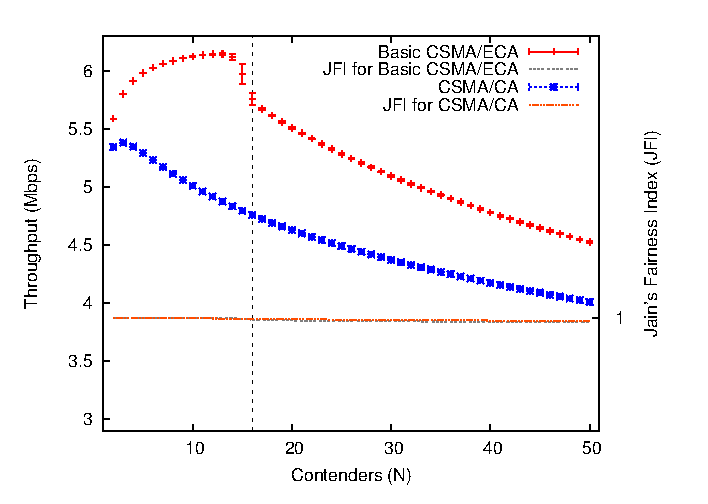
\includegraphics[width=\linewidth]{ECA-vs-CA-FINAL.eps}}
	\fi
	(0,-4.15) node {\smaller Throughput and fairness in CSMA/CA and Basic CSMA/ECA.};
\end{tikzpicture}
\end{center}

Nevertheless, when the number of contenders surpasses $CW_{\min}/2$, the system incurs in a mixed behavior; some nodes pick a random and others a deterministic backoff counter. This setup has undesired repercussion in the attained throughput, approximating Basic ECA's to CSMA/CA's.

}

% \headerbox{Throughput and fairness in CSMA/CA and CSMA/ECA}{name=throughputBasicECA,column=0,below=hysteresis,above=bottom}{
% 
% Explaining why the throughput figures look as they do.
% 
% Also it is worth to mention the fair nature of both protocols.
% \begin{center}
% \begin{tikzpicture}
% \path
% 	\ifpdf
% 		(0,0) node{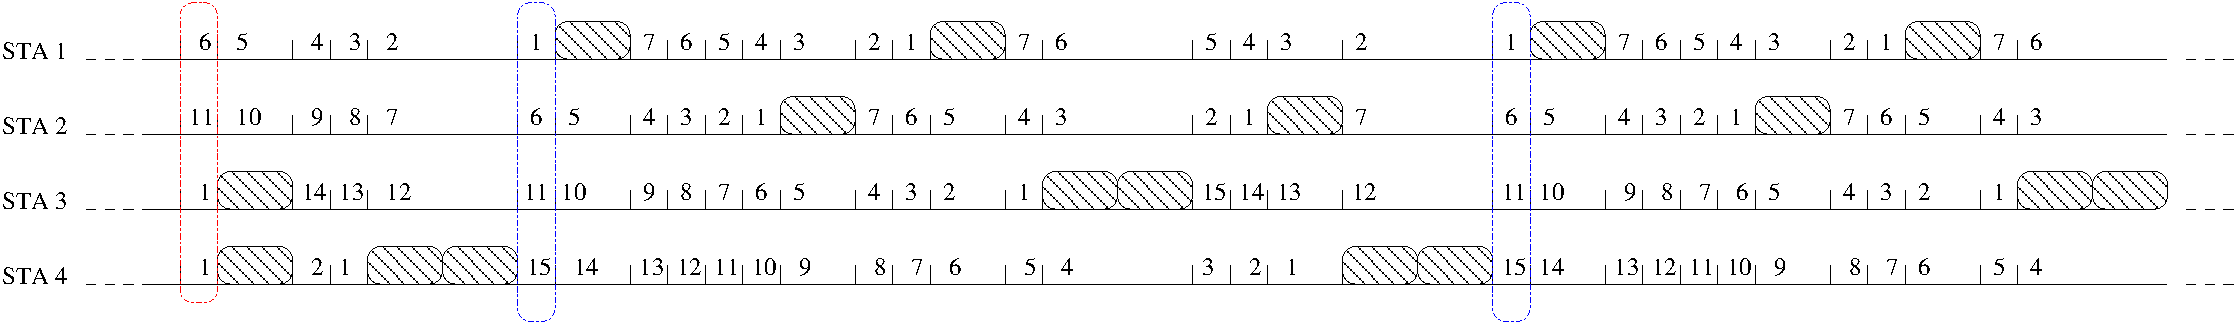
\includegraphics[width=\linewidth]{csma_eca_different_backoff-eps-converted-to.pdf}}
% 	\else
% 		(0,0) node{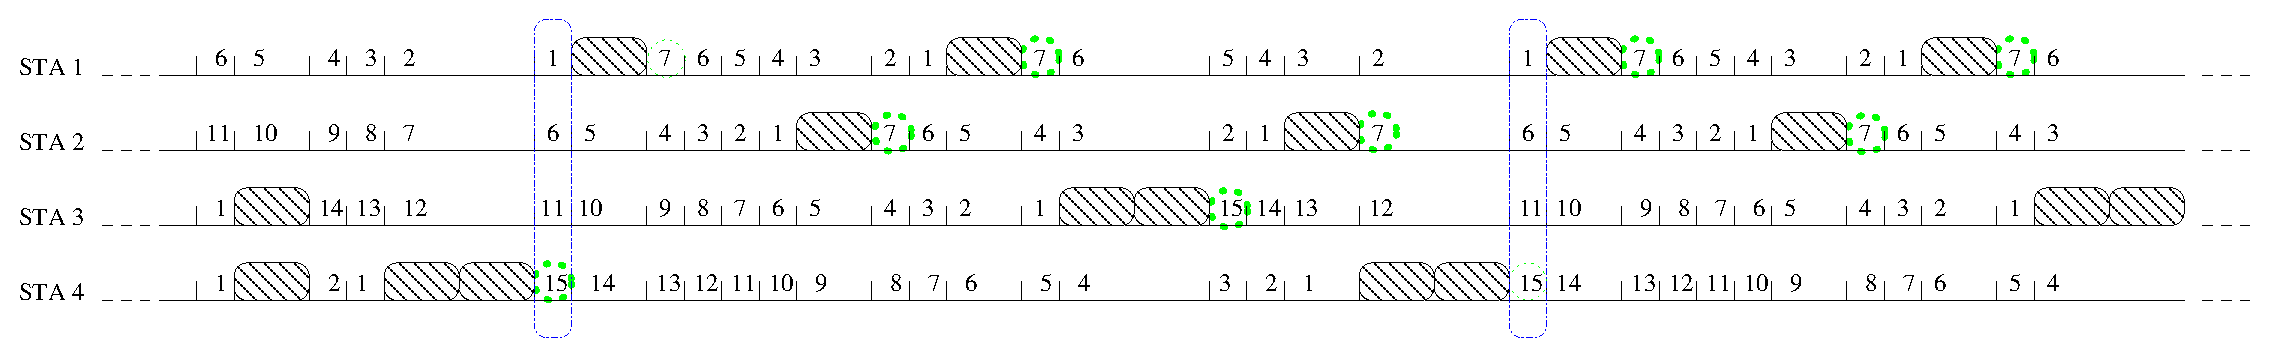
\includegraphics[width=\linewidth]{csma_eca_different_backoff.eps}}
% 	\fi
% 	(0,-1.0) node {\smaller Example CSMA/ECA behavior.};
% \end{tikzpicture}
% \end{center}
% 
% }

\headerbox{CSMA/ECA + hysteresis and fair share}{name=fullECA,column=1,span=1,below=motivation}{

Explanation on how the hysteresis allows us to support many more contenders in a collision-free fashion. And also how fair share corrects the unfairness issue associated with hysteresis.

\begin{center}
\begin{tikzpicture}
\path
	\ifpdf
		(0,0) node{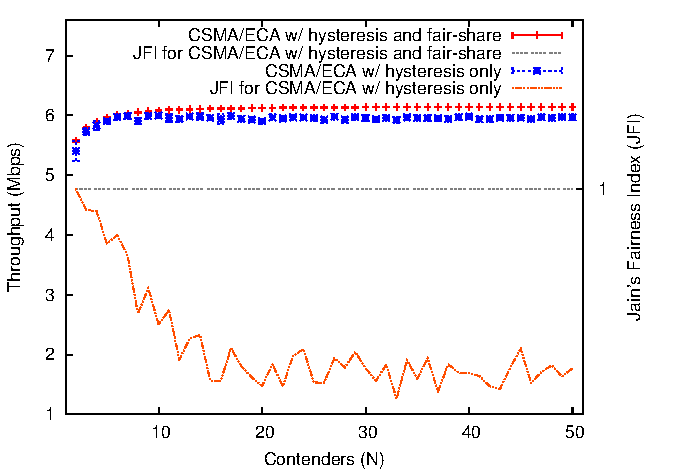
\includegraphics[width=\linewidth]{ECA-w-enhancements-FINAL-eps-converted-to.pdf}}
	\else
		(0,0) node{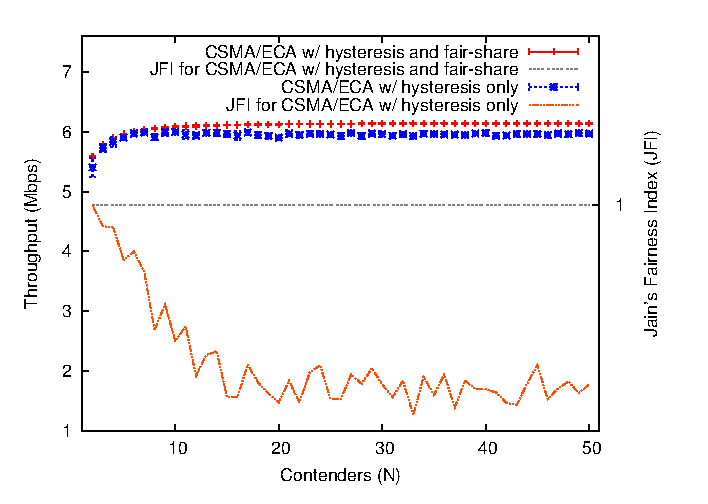
\includegraphics[width=\linewidth]{ECA-w-enhancements-FINAL.eps}}
	\fi
	(0,-4.2) node {\smaller An STB establishes active (used) and inactive (unused) SIP sessions.};
\end{tikzpicture}
\end{center}

}

\headerbox{Future plans}{name=future,column=1,below=fullECA}{

Some of the future directions of the project:
\begin{itemize}
	\item Unsaturated scenarios.
	\item To implement IEEE 802.11e EDCA.
	\item Wireless MAC Processors.
	\item Implementation in RFID networks.
\end{itemize}

\begin{center}
\begin{tikzpicture}
\path
	\ifpdf
		(0,0) node{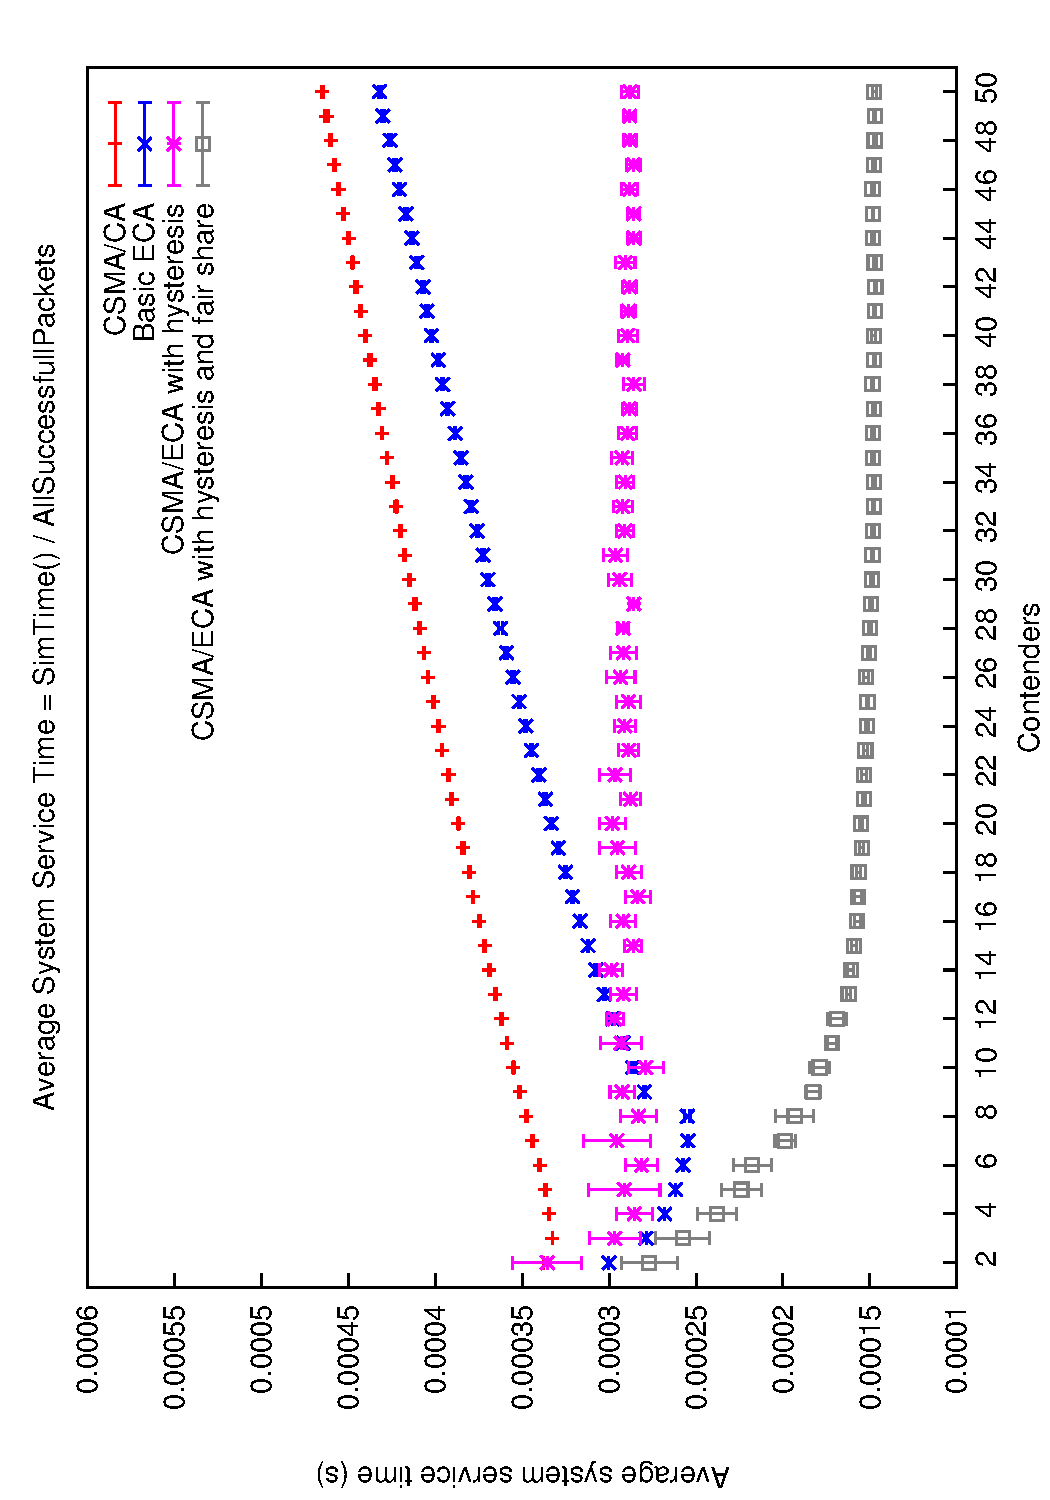
\includegraphics[width=0.5\linewidth, angle=-90]{avgSystemServiceTime-eps-converted-to.pdf}}
	\else
		(0,0) node{\includegraphics[width=0.5\linewidth]{avgSystemServiceTime.eps}}
	\fi
	(0,-3.2) node {\smaller Average system service time.};
\end{tikzpicture}
\end{center}
}

\headerbox{References}{name=references,span=1,column=1,above=bottom}{

{
% \scriptsize
% 
% \renewcommand*{\refname}{\vspace*{-0.5em}}
% \let\oldbibliography\thebibliography
% \renewcommand{\thebibliography}[1]{\oldbibliography{#1}\setlength{\itemsep}{-0.3em}}

\bibliographystyle{Classes/IEEEtran}
\bibliography{IEEEabrv,ref}

% \begin{thebibliography}{1}
% 
% \bibitem{bikfalvi2009ijcs}
% Alex Bikfalvi, Jaime Garc\'{i}a-Reinoso, Iv\'{a}n Vidal, and Francisco Valera.
% \newblock A peer-to-peer iptv service architecture for the ip multimedia
%   subsystem.
% \newblock {\em International Journal of Communication Systems},
%   23(6--7):780--801, June--July 2009.
% 
% \bibitem{qiu2009modelinguser}
% T.~Qiu, Z.~Ge, S.~Lee, J.~Wang, J.~Xu, and Q.~Zhao.
% \newblock Modeling user activities in a large iptv system.
% \newblock In {\em Proceedings of the 9th ACM SIGCOMM conference on Internet
%   measurement conference}, pages 430--441. ACM, 2009.
% 
% \bibitem{qiu2009modelingchannel}
% T.~Qiu, Z.~Ge, S.~Lee, J.~Wang, Q.~Zhao, and J.~Xu.
% \newblock Modeling channel popularity dynamics in a large iptv system.
% \newblock In {\em Proceedings of the eleventh international joint conference on
%   Measurement and modeling of computer systems}, pages 275--286. ACM, 2009.
% 
% \end{thebibliography}
}

}

\end{poster}

\end{document}
